\documentclass[a4paper, 14pt]{extreport}
\usepackage[T2A]{fontenc}
\usepackage[utf8]{inputenc}
\usepackage[english, russian]{babel}
\usepackage{indentfirst}
\usepackage{setspace}
\usepackage{titlesec}
\usepackage{subcaption}
\usepackage{hyperref}
\usepackage[left=2.5cm, right=1.5cm, top=2.0cm, bottom=2.0cm]{geometry}
\usepackage{graphicx}
\graphicspath{{images/}}

\renewcommand{\rmdefault}{ftm}

\titleformat{\chapter}
    {\centering\normalsize}
    {\thechapter}
    {8pt}{\MakeUppercase}
\titleformat{\section}
    {\centering\normalsize}
    {\thesection}
    {1em}{}
\titleformat{\subsection}
    {\centering\normalsize}
    {\thesubsection}
    {1em}{}
\titlespacing*{\chapter}{0pt}{-30pt}{8pt}
\titlespacing*{\section}{\parindent}{*4}{*4}
\titlespacing*{\subsection}{\parindent}{*4}{*4}

\begin{document}
    \begin{titlepage}
        \begin{center}
            Министерство образования и науки РФ \\
            Государственное образовательное учреждение\\
            Высшего профессионального образования\\
            <<Волгоградский государственный технический университет>>\\
            Кафедра <<САПР и ПК>>
        \end{center}
        \vspace{2.0cm}
        \begin{center}
            \large \textbf{ОТЧЁТ} \\
            по педагогической практике
        \end{center}
        \begin{flushleft}
            Студента\\
            Фамилия \underline{\hspace{5cm}} 
            Имя \underline{\hspace{5.1cm}}\\
            Отчество \underline{\hspace{5cm}}\\
            Факультет \underline{\hspace{4.8cm}} курс \underline{\hspace{2cm}} 
            группа \underline{\hspace{4cm}}\\
        \end{flushleft}
        \vspace{1.0cm}
        \noindentТема работы: \underline{\hspace{10cm}}
        \vspace{2.0cm}
        \begin{flushleft}
            РУКОВОДИТЕЛЬ ПРАКТИКИ\\
            Кафедра \underline{\hspace{5cm}} Должность \underline{\hspace{5cm}} \\
            Фамилия \underline{\hspace{4.9cm}} Имя \underline{\hspace{6.5cm}}\\
            Отчество \underline{\hspace{4.9cm}}
        \end{flushleft}
        \vspace{1.5cm}
        \begin{flushright}
            <<\underline{\hspace{1.0cm}}>>\underline{\hspace{4.0cm}} \the\year г.
        \end{flushright}
        \vspace{\fill}
        \begin{center}
            Волгоград \the\year
        \end{center}
    \end{titlepage}
    \tableofcontents
    \onehalfspacing
    \chapter{Описание методических указаний к лабораторной работе}
    VirtualBox~--- программный продукт нативной виртуализации, разработанный
    компаниями Innotek, Sun Microsystems и Oracle. Продукт является
    кроссплатформенным, поддерживает виртуализации различных устройств,
    различные виды сетевых взаимодействий, аппаратное 3D-ускорение.

    Цель методических указаний~-- ознакомить студента с видами виртуализации
    и научить основам работы с Oracle VM VirtualBox.

    После выполнения лабораторной работы студент получит:
    \begin{itemize}
        \item представление о технологиях виртуализации;
        \item навыки работы с VirtualBox;
        \item навыки работы с ОС Ubuntu Linux.
    \end{itemize}
    
    Разработанные методические указания позволят студенту разобраться в
    типах виртуализации, созданию и настройке виртуальных машин с помощью
    VirtualBox и использовать этот программный продукт для собственных нужд.

    В каждом из разделов подробно описана та или иная функциональная
    возможность виртуальных машин или Oracle VM VirtualBox в целом.

    \chapter{Сбор информации}
    Информация по технологиям виртуализации и VirtualBox была собрана из
    различных интернет источников. Самая актуальная и достоверная информация,
    среди которой: виды виртуализации, примеры использования виртуальных машин,
    настройка виртуальных машин VirtualBox, была взята со следующих сайтов:
    \begin{itemize}
        \item Хабрахабр -- многофункциональный сайт, представляющий собой
            смешение новостного сайта и коллективного блога, созданный для
            публикации новостей, аналитических статей, мыслей, связанных с
            информационными технологиями, бизнесом и Интернетом.\\
            \url{http://habrahabr.ru/}
        \item iXBT.com -- специализированный российский
            информационно-аналитический сайт с новостями из сферы IT,
            детальными обзорами техники и программного обеспечения.
            \url{http://www.ixbt.com/}
        \item Ubuntu -- Open-Source операционная система на базе Debian
            GNU/Linux.\\
            \url{http://ubuntu.ru/}
        \item Wikipedia -- свободная общедоступная мультиязычная
            универсальная ин\-тер\-нет-энциклопедия, реализованная на принципах
            Вики.\\
            \url{https://ru.wikipedia.org}
    \end{itemize}
    
    К одним из основных источников информации можно причислить Хабрахабр, так
    как в его тематических блогах имеется большое количество информации
    предоставляющее подробное объяснение по тому или иному вопросу. Стоит также
    выделить хороший стиль подачи информации и подкрепление текста визуальной
    информацией.

    \chapter{Структура методических указаний}
    В структуре методических указаний были выделены следующие пункты:
    \begin{enumerate}
        \item Цель, задачи
        \item Теоретические положения
        \begin{enumerate}
            \item Виртуализация и виртуальные машины
            \item Виды виртуализации
            \begin{enumerate}
                \item Визуализация платформ
                \item Визуализация ресурсов
            \end{enumerate}
            \item Oracle VM VirtualBox
            \begin{enumerate}
                \item Ключевые возможности
                \item Примеры использования
            \end{enumerate}
        \end{enumerate}
        \item Пример выполнения лабораторной работы
        \begin{enumerate}
            \item Подготовка к запуску виртуальной машины
            \item Запуск готовой виртуальной машины
            \item Установка VirtualBox
            \item Создание виртуальной машины
            \item Запуск созданной виртуальной машины
        \end{enumerate}
        \item Задания на выполнение лабораторной работы
        \item Контрольные вопросы
        \item Литература
    \end{enumerate}

    \newpage

    В разделе <<Цель, задачи>> приводится цель лабораторной работы и общие
    задачи, которые студент должен сделать во время ее выполнения.

    В разделе <<Теоретические положения>> даётся общее описание технологии
    виртуализации и описание видов виртуализации. Так же в этом разделе дается
    описание программного продукта Oracle VM VirtualBox и его ключевые
    возможности.

    В разделе <<Пример выполнения лабораторной работы>> студенту
    предоставляется пример создания, настройки и запуска витруальной машины
    с помощью VirtualBox в ОС Ubuntu Linux. Все действия снабжены подробным
    описанием и снимками экрана.

    В разделе <<Задания на выполнение лабораторной работы>> представлены
    типовые задания для закрепления изученного материала лабораторной работы.

    В разделе <<Контрольные вопросы>>~-- контрольные вопросы для проверки
    теоретического минимума по данной теме.
    
    Исходный код методических указаний доступен по следующей ссылке:\\
    \url{https://github.com/vstu-cad-stuff/vbox-manual}


    \chapter{Скриншоты работы с Oracle VM VirtualBox}
    \begin{figure}[ht!]
        \center
        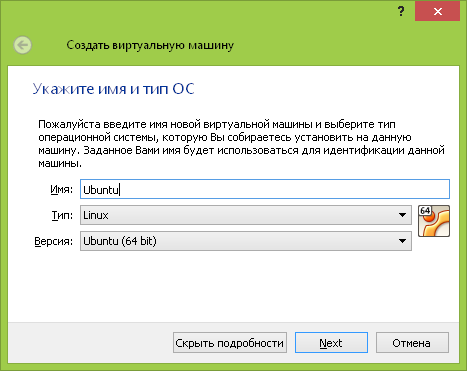
\includegraphics[width=.6\textwidth]{vbox_02} \\[.5em]
        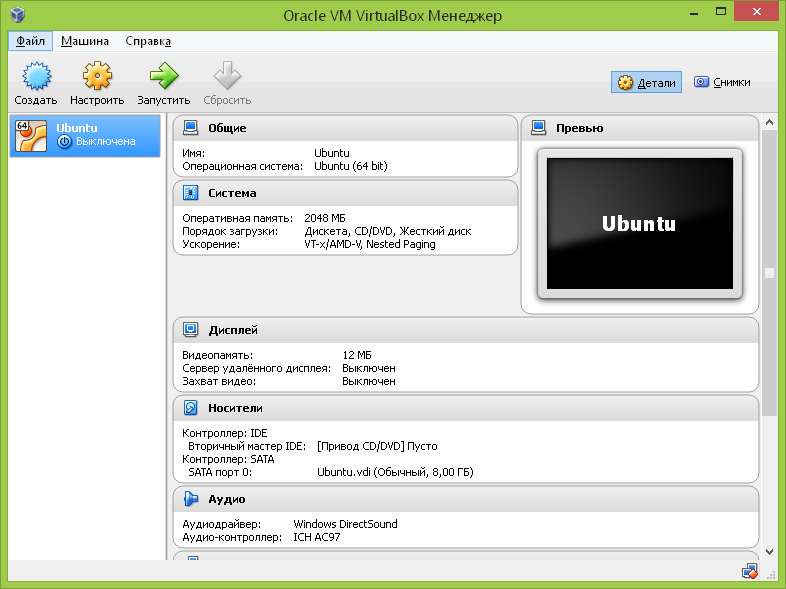
\includegraphics[width=.6\textwidth]{vbox_08} \\[.5em]
        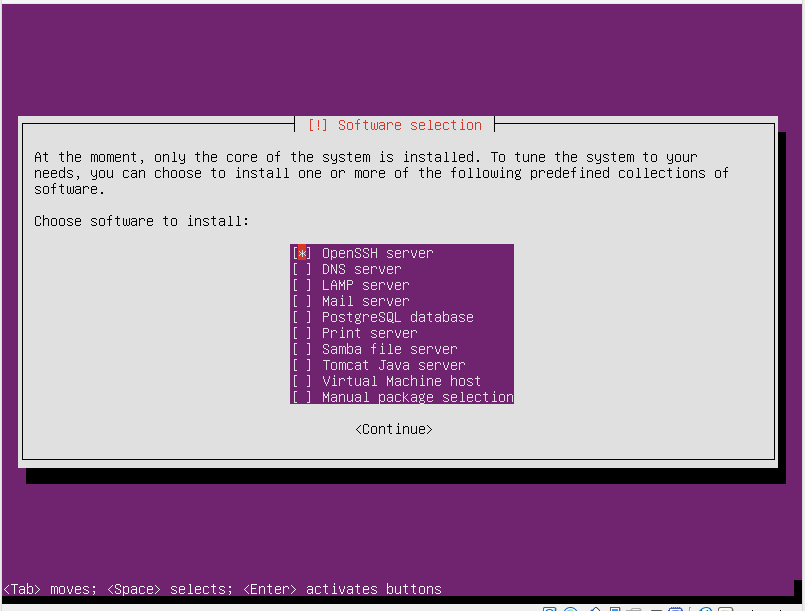
\includegraphics[width=.6\textwidth]{vbox_10}
    \end{figure}

    \chapter{Используемые технологии}
    Для проектирования и вёрстки были использованы следующие свободно распространяемые программные 
    продукты:
    \begin{itemize}
        \item Ubuntu Linux -- это i686/x86-64 дистрибутив GNU/Linux общего 
            назначения, разрабатываемый на основе Debian.\\
            \url{http://www.ubuntu.ru/}
        \item Oracle VM VirtualBox -- программный продукт виртуализации для
            различных операционных систем.\\
            \url{https://www.virtualbox.org/}
        \item \TeX -- система компьютерной вёрстки, разработанная американским профессором информатики 
            Дональдом Кнутом в целях создания компьютерной типографии.\\
            \url{http://tug.org/}
        \item \LaTeX -- набор макрорасширений системы компьютерной вёрстки TeX.\\
            \url{http://www.latex-project.org/}
        \item Sublime Text 3 -- быстрый кроссплатформенный редактор исходных текстов программ.\\
            \url{www.sublimetext.com/3}
            
        \item Mozilla Firefox -- свободный браузер на движке Gecko, разработкой и распространением 
            которого занимается Mozilla Corporation.\\
            \url{https://www.mozilla.org/}
        \item Git -- распределённая система управления версиями файлов. Проект был создан Линусом 
            Торвальдсом для управления разработкой ядра Linux, первая версия выпущена 7 апреля 2005 года.\\
            \url{http://git-scm.com/}
        \item GitHub -- самый крупный веб-сервис для хостинга IT-проектов и их совместной разработки. 
            Основан на системе контроля версий Git и разработан на Ruby on Rails и Erlang компанией 
            GitHub, Inc.\\
            \url{https://github.com/}
    \end{itemize}
\end{document}